\section{System design}
In this section, the requirement and tasks are discussed. Over past 12 month, we closely worked with two domain researchers in urban air quality analysis and forecast. One researcher(R1) is in the field of the atmospheric diffusion of air pollutants, the other researcher(R2) is working on the air pollutant forecast through machine learning techniques. Both of them has strong domain experience in the air quality forecast. 


\zw{what's differences between design goals and tasks?
so many goals and tasks? what are their relationships?}


\subsection{Design Goals}
We have distilled the following goals based on an informal interview with domain experts who work on utilizing RNN models to predict weather pollution.

\textbf{G1: Analyze RNN from different perspectives and scales.} 
Understanding and interpreting RNN models require users to examine the model from different perspectives and at different scales.
For example, showing the activation patterns of the hidden units can provide users an overview on model parameter utilization.
Looking at the features and model results can help users understand what are the most critical factors in prediction.
Examining data similarities can also enable users to quickly drill down to their points of interest.
Each perspective has its unique value and users usually require to switch between different perspectives during model exploration and interpretation.
In addition, it is also important to understand RNN models at different scales during exploration.
From a high-level analysis, users may need to first obtain a data overview to inspect if there's any abnormal data patterns.
Summarizing the value distribution of hidden states can also demonstrate an overall model behavior pattern.
From a finer granularity, users may drill down to looking into a particular sequence for prediction details and identifying the most influential features or time steps.
Therefore, the visualization system needs to enable users exploring RNN at different scales.

\textbf{G2: Reveal information captured by the model.} 
To understand and interpret model's prediction, it is necessary to reveal what information is captured by RNN models.
This information can facilitate users to determine whether the predictions are trustful and examine whether the model misses any important domain factors or learns any insights.
To achieve this, the visualization not only needs to provide model parameter information such as hidden state statistics but also requires to link the parameters to the input features so that users can know what prediction behaviors are captured by different hidden units.
For example, from the activation distribution of the hidden units, users can estimate what percentage of hidden units are usually active, thus determine whether the model's capacity is enough to distinguish the variety of data.
By calculating how different features can activate a certain hidden state, users can learn to what factors the model pay attention and what are the most influential features for prediction.
Furthermore, analyzing the hidden states that are passed between consecutive time steps also enable users to inspect what historical information is helpful for prediction and to identify the important time steps.
Thus, revealing the information captured by RNN models can directly facilitate model interpretation.

\textbf{G3: Support case-based exploration.} 
Case-based exploration is one of the most effective strategies for humans to interpret machine learning models.
It is based on the assumption that a new problem can be resolved by the solutions of previous similar problems, which can serve as a scaffold for understanding the challenges.
Adopting case-based exploration can facilitate users to obtain an overview on RNN models such as observing which types of data the model tends to make errors or identifying the most critical features that can affect a prediction. 
Users can compare two similar sequences to see if the model performance is consistent or examine the predictions at consecutive time steps to estimate when the model's behavior changes dramatically.
However, providing case-based exploration for RNN models is challenging as the system needs to flexible enough for users to filter and search the cases of interests.
To examine a case, which consists of high-dimensional vectors from multiple time steps, the system is also required to be scalable and able to provide informative summarization at the same time.
We aim to provide users a flexible and effective case-based exploration work-flow.

\subsection{Analytical Tasks}
To fulfill the aforementioned design goals, we have distilled the following analytical tasks:

\textbf{T1: Encode hidden state statistics.}
Hidden states, a direct reflection of model's intermediate results, is critical for revealing the information captured by a model (\textbf{G1, G2}).
Visualizing hidden state statistics can provide an holistic picture of model's capacity and behavior.
For example, summarizing the overall activeness of all the hidden units can help users estimate whether the current parameter size is appropriate.
By linking the hidden state activeness with data and prediction results, users can also identify the blind points where models tend to predict incorrectly.
Thus, our system should support encode various hidden state statistics such as value distribution and the data coverage.

\textbf{T2: Encode feature statistics.}
Apart from hidden states, feature statistics are another perspective for improving model performance.
First, analyzing feature value distribution can help understand feature dependency, from which domain experts can remove redundant features and improve model efficiency.
In a detailed examination of one particular sequence, visualizing the input features at different time steps can also make users understand at which time step the input changes dramatically to avoid misinterpretation on prediction results.
We aim to provide feature statistics at different scales (\textbf{G1, G2}).

\textbf{T3: Analyze relationships between features and hidden states.}
In addition to visualize the hidden states and features individually, analyzing the relationships between features and hidden states can further help users understand what patterns are captured by the model (\textbf{G1, G2}).
By inspecting what features can activate certain hidden units, users can know how the model pays attention to different factors and how to aggregate these information to generate the final prediction.
This also enable users to see if the model has utilized all the features or only focus on the most important ones.
This requires the system to link the features together with hidden states and visualize their relationships clearly.

\textbf{T4: Support temporal analysis.}
One major advantage of RNN models is that they can capture time-dependent sequence information.
The prediction is affected not only by the features from the last time step, but also the historical information being passed along the sequence.
Showing what information is reserved along the sequence and what information is discarded helps users better understand how the temporal information is utilized by the model (\textbf{G1, G2}).
In addition, users can also identify the most critical time step that causes a dramatic change in the model's prediction.
For these reasons, the system should be able to support temporal analysis when interpreting model's behaviors.

\textbf{T5: Identify data clusters and outliers.}
To support case-based reasoning, users need to first obtaining a data overview by identifying the data clusters and outliers (\textbf{G1, G3}).
This provides concrete examples to guide users to further explore the data of interests.
For example, users can estimate how many categories of data sharing the same or similar prediction results by observing data clusters.
Users can also inspect the outliers that have distinct prediction results to detect if the model behave incorrectly according to certain domain knowledge.
We aim to provide users an overview on data and enable them to compare different data and their prediction results.

\textbf{T6: Enable sequence comparison.}
As the key concept of case-based exploration is to use existing knowledge to solve similar new problems, enabling sequence comparison is necessary in interpreting RNN models (\textbf{G1, G3}).
Many use scenarios require users to compare the prediction processes of multiple sequences at the same time.
For example, users may need to examine two similar but slightly different sequences to identify at which time steps the model behave differently.
Conversely, users may also compare multiple sequences with similar prediction results to identify their common features.
Therefore, the system needs to enable sequence comparison in different perspectives including both the hidden states and raw features.

\textbf{T7: Support interactive model exploration}.
All the tasks listed above require the system to provide interactive model exploration.
For example, users may filter certain hidden states and want to inspect the features that can only activate these selected hidden states.
Users may also need to select a few interested sequences for comparison and focus on certain time steps.
These requirements need to system to support a set of interactions for interactive exploration.




\subsection{System Overview}

\begin{figure}[t]
	\centering
    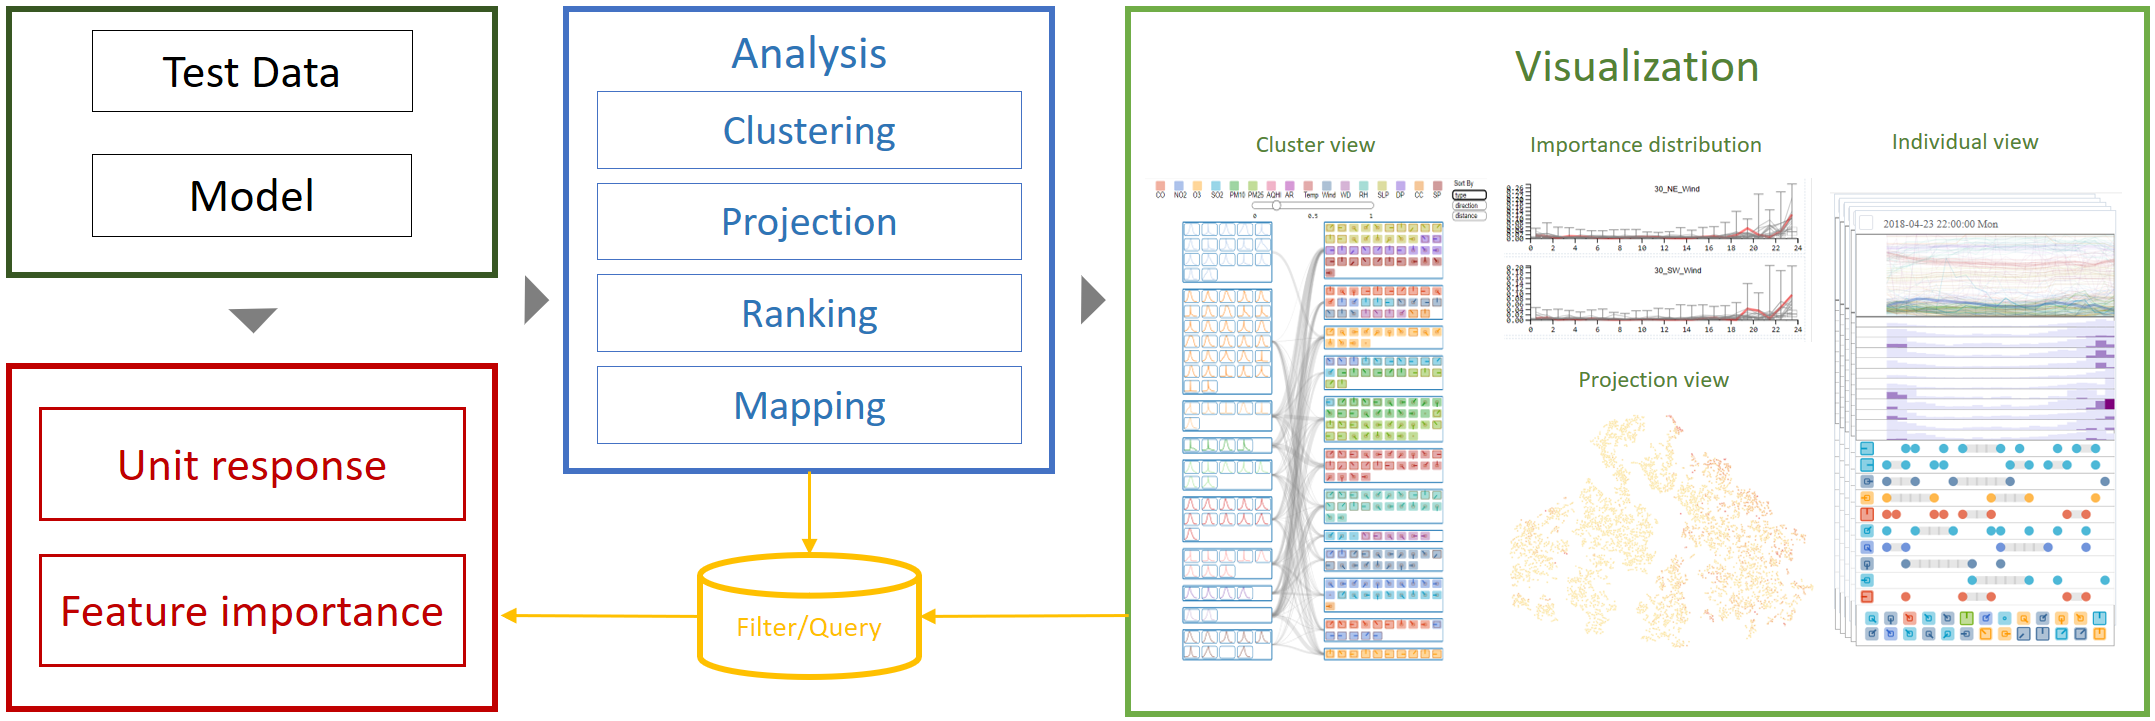
\includegraphics[width=0.45\textwidth]{pictures/System_framework.png}
	\vspace{-3mm}
	\caption{System framework}
	\label{fig:system_framework}
	\vspace{-4mm}
\end{figure}

In this section, the system overview are discussed as Fig ~\ref{fig:system_framework}. The whole system consists of three components: model manager, model interpreter and visualization. 

The model manager is designed to manipulate trained models and enable users to select the dataset they are interested in. With a choosing model and dataset, the model manager will manage the input data, output of each hidden states, and the gradient of input with respect to the hidden states output into the files.    

With the output of model manager, then the model interpreter calculates the distribution of hidden states output first. Then it extracts the correlation graph by analyzing the difference of these distributions. At last, the model interpreter discover the dependency relations between the hidden state through the input gradient which will be discussed in section 5. 

The distribution, correlation graph and dependency table will be finally provided to the visualization module. The visualization~\ref{fig:teaser} has six components, the control panel enable users to select the test data, trained model and configure parameters. The cluster view visualize the overview relationship between the variables and hidden units, users are allowed to interactively verify if a pattern is captured by the RNN model. The projection view projects the filtered sequence by using tsne which allow users identify how the hidden states are able to \QM{distinguish the different patterns}. The sequence view enable users to explore the data at individual level, where the temporal dependency between each hidden states and the dependency between the hidden states and input data will be visualized. All views are linked when common items are selected. 

